\documentclass[a4paper]{report}
\usepackage{a4wide}
\usepackage[utf8]{inputenc}
\usepackage[T1]{fontenc}
\usepackage{parskip}
\usepackage{hyperref}
\usepackage{epsfig}
\usepackage{background}
\usepackage{mathptmx}

% To avoid tikz error, see https://tex.stackexchange.com/questions/165929/semiverbatim-with-tikz-in-beamer
\makeatletter
\global\let\tikz@ensure@dollar@catcode=\relax
\makeatother

\backgroundsetup{
scale=1,
angle=0,
opacity=1,
contents={
\includegraphics[width=\paperwidth,height=\paperheight]{images/spi-front.jpg}}
}

\hypersetup{
  colorlinks   = true,
  urlcolor     = blue,
  linkcolor    = blue,
  pdfinfo = {
    Title = {SPI Annual Report 2022},
    Author = {Software in the Public Interest, Inc.},
    Keywords = {SPI, free software, open source, FOSS, annual report, charity, non-profit, 501c3},
  }
}

\begin{document}

\title{Software in the Public Interest, Inc.\\
2022 Annual Report}
\date{July XX, 2023}

\maketitle

\newpage

\backgroundsetup{
scale=1,
angle=0,
opacity=1,
contents={
\includegraphics[width=\paperwidth,height=\paperheight]{images/spi-content.jpg}}
}

\hspace{1em}

To the membership, board and friends of Software in the Public Interest, Inc:

As mandated by Article 8 of the SPI Bylaws, I respectfully submit this annual report on the activities of Software in the Public Interest, Inc. and extend my thanks to all of those who contributed to the mission of SPI in the past year.

  \emph{-- Michael Schultheiss, SPI President}

\newpage

\tableofcontents

\newpage

\chapter{President's Welcome}
\label{sec:president}

  \emph{-- Michael Schultheiss, SPI President}

\chapter{Committee Reports}
\section{Membership Committee}

\subsection{Statistics}

On January 1, 2022 we had 243 contributing and 1253 non-contributing members.  On December 31, 2022 there were 258 contributing members and 1299 non-contributing members.  This is an increase of 15 contributing members and an increase of 46 non-contributing members.

\chapter{Board Report}
\section{Board Members}

Board members as of January 1, 2022:

\begin{itemize}
\item Michael Schultheiss (President)
\item Stephen Frost (Vice President)
\item Tim Potter (Secretary)
\item Héctor Orón Martínez (Treasurer)
\item Joe Conway
\item Forrest Fleming
\item Milan Kupcevic
\item Chris Lamb
\item Martin Zobel-Helas
\end{itemize}

Board members as of December 31, 2022:

\begin{itemize}
\item Michael Schultheiss (President)
\item Stephen Frost (Vice President)
\item Forrest Fleming (Secretary)
\item Héctor Orón Martínez (Treasurer)
\item Joe Conway
\item Milan Kupcevic
\item Jonatas L. Nogueira
\item Jeremy Stanley
\item Zach van Rijn
\end{itemize}

\section{Board Changes}

Changes that occurred during the year:

\begin{itemize}

\item The terms for Forrest Fleming, Chris Lamb, Héctor Orón Martínez, and Martin Zobel-Helas expired in July 2022.  Tim Potter stepped down from the board.  Forrest and Héctor sought, and obtained, re-election.  We'd like to thank Chris, Martin and Tim for their work on the board.  Jonatas L. Nogueira, Jeremy Stanley, and Zach van Rijn joined the board as part of the same election.

\item On August 8, 2022 the board voted to appoint the following officers:

\begin{itemize}
\item President: Michael Schultheiss
\item Vice President: Stephen Frost
\item Secretary: Forrest Fleming
\item Treasurer: Héctor Orón Martínez
\end{itemize}

\end{itemize}

\section{Elections}

A board membership election was conducted in July 2022.  There were 5 board seats up for election.  Nominations were received from Forrest Fleming, Jonatas L. Nogueira, Héctor Orón Martínez, Zach van Rijn, and Jeremy Stanley.  Since there were 5 nominations for 5 board seats, no vote was required and all three candidates were elected for a 3 year term.

\chapter{Treasurer's Report}

\chapter{Member Project Reports}

\section{New Associated Projects}

\subsection{Battle for Wesnoth}

\href{https://www.wesnoth.org/}{Battle for Wesnoth} is an open source, turn-based strategy game with a high fantasy theme. It features both single-player and online/hotseat multiplayer combat. The game also allows its users to create their own ``campaigns'' and make them publicly available, as well as collaborating with the core team to expand the open source gaming ecosystem.

\subsection{MPI Forum}

The \href{https://www.mpi-forum.org/}{MPI Forum} is the standardization body for the Message Passing Interface (MPI), a hardware agnostic interface for passing messages for parallel and distributed computing. MPI is implemented in a number of open-source and proprietary libraries and widely used in academic, corporate, and research institutions. The MPI Forum meets regularly to discuss and design the next version of the MPI Standard. The work of the MPI Forum happens in our public GitHub repositories, and anyone is welcome to participate by joining the MPI Forum's mailing list and attending our virtual and physical meetings.

\section{Projects No Longer Associated with SPI}

\begin{itemize}

\item Chakra Linux is no longer active.

\item Glucosio is no longer active.

\end{itemize}

\section{Updates from Associated Projects}



\appendix
\chapter{About SPI}

SPI is a non-profit organization which was founded to help organizations develop and distribute open hardware and software. We encourage programmers to use the GNU General Public License or other licenses that allow free redistribution and use of software, and hardware developers to distribute documentation that will allow device drivers to be written for their product.

SPI was incorporated as a non-profit organization on June 16, 1997 in the state of New York. Since then, it has become an umbrella organization for projects from the community.

In 1999, the Internal Revenue Service (IRS) of the United States government determined that under section 501(a) of the Internal Revenue Code SPI qualifies for 501(c)(3) (non-profit organization) status under section 509(a)(1) and 170(b)(1)(A)(vi). This means that donations made to SPI and its supported projects are tax-deductible as charitable donations for US taxpayers.

\newpage

\pagestyle{empty}

\backgroundsetup{
scale=1,
angle=0,
opacity=1,
contents={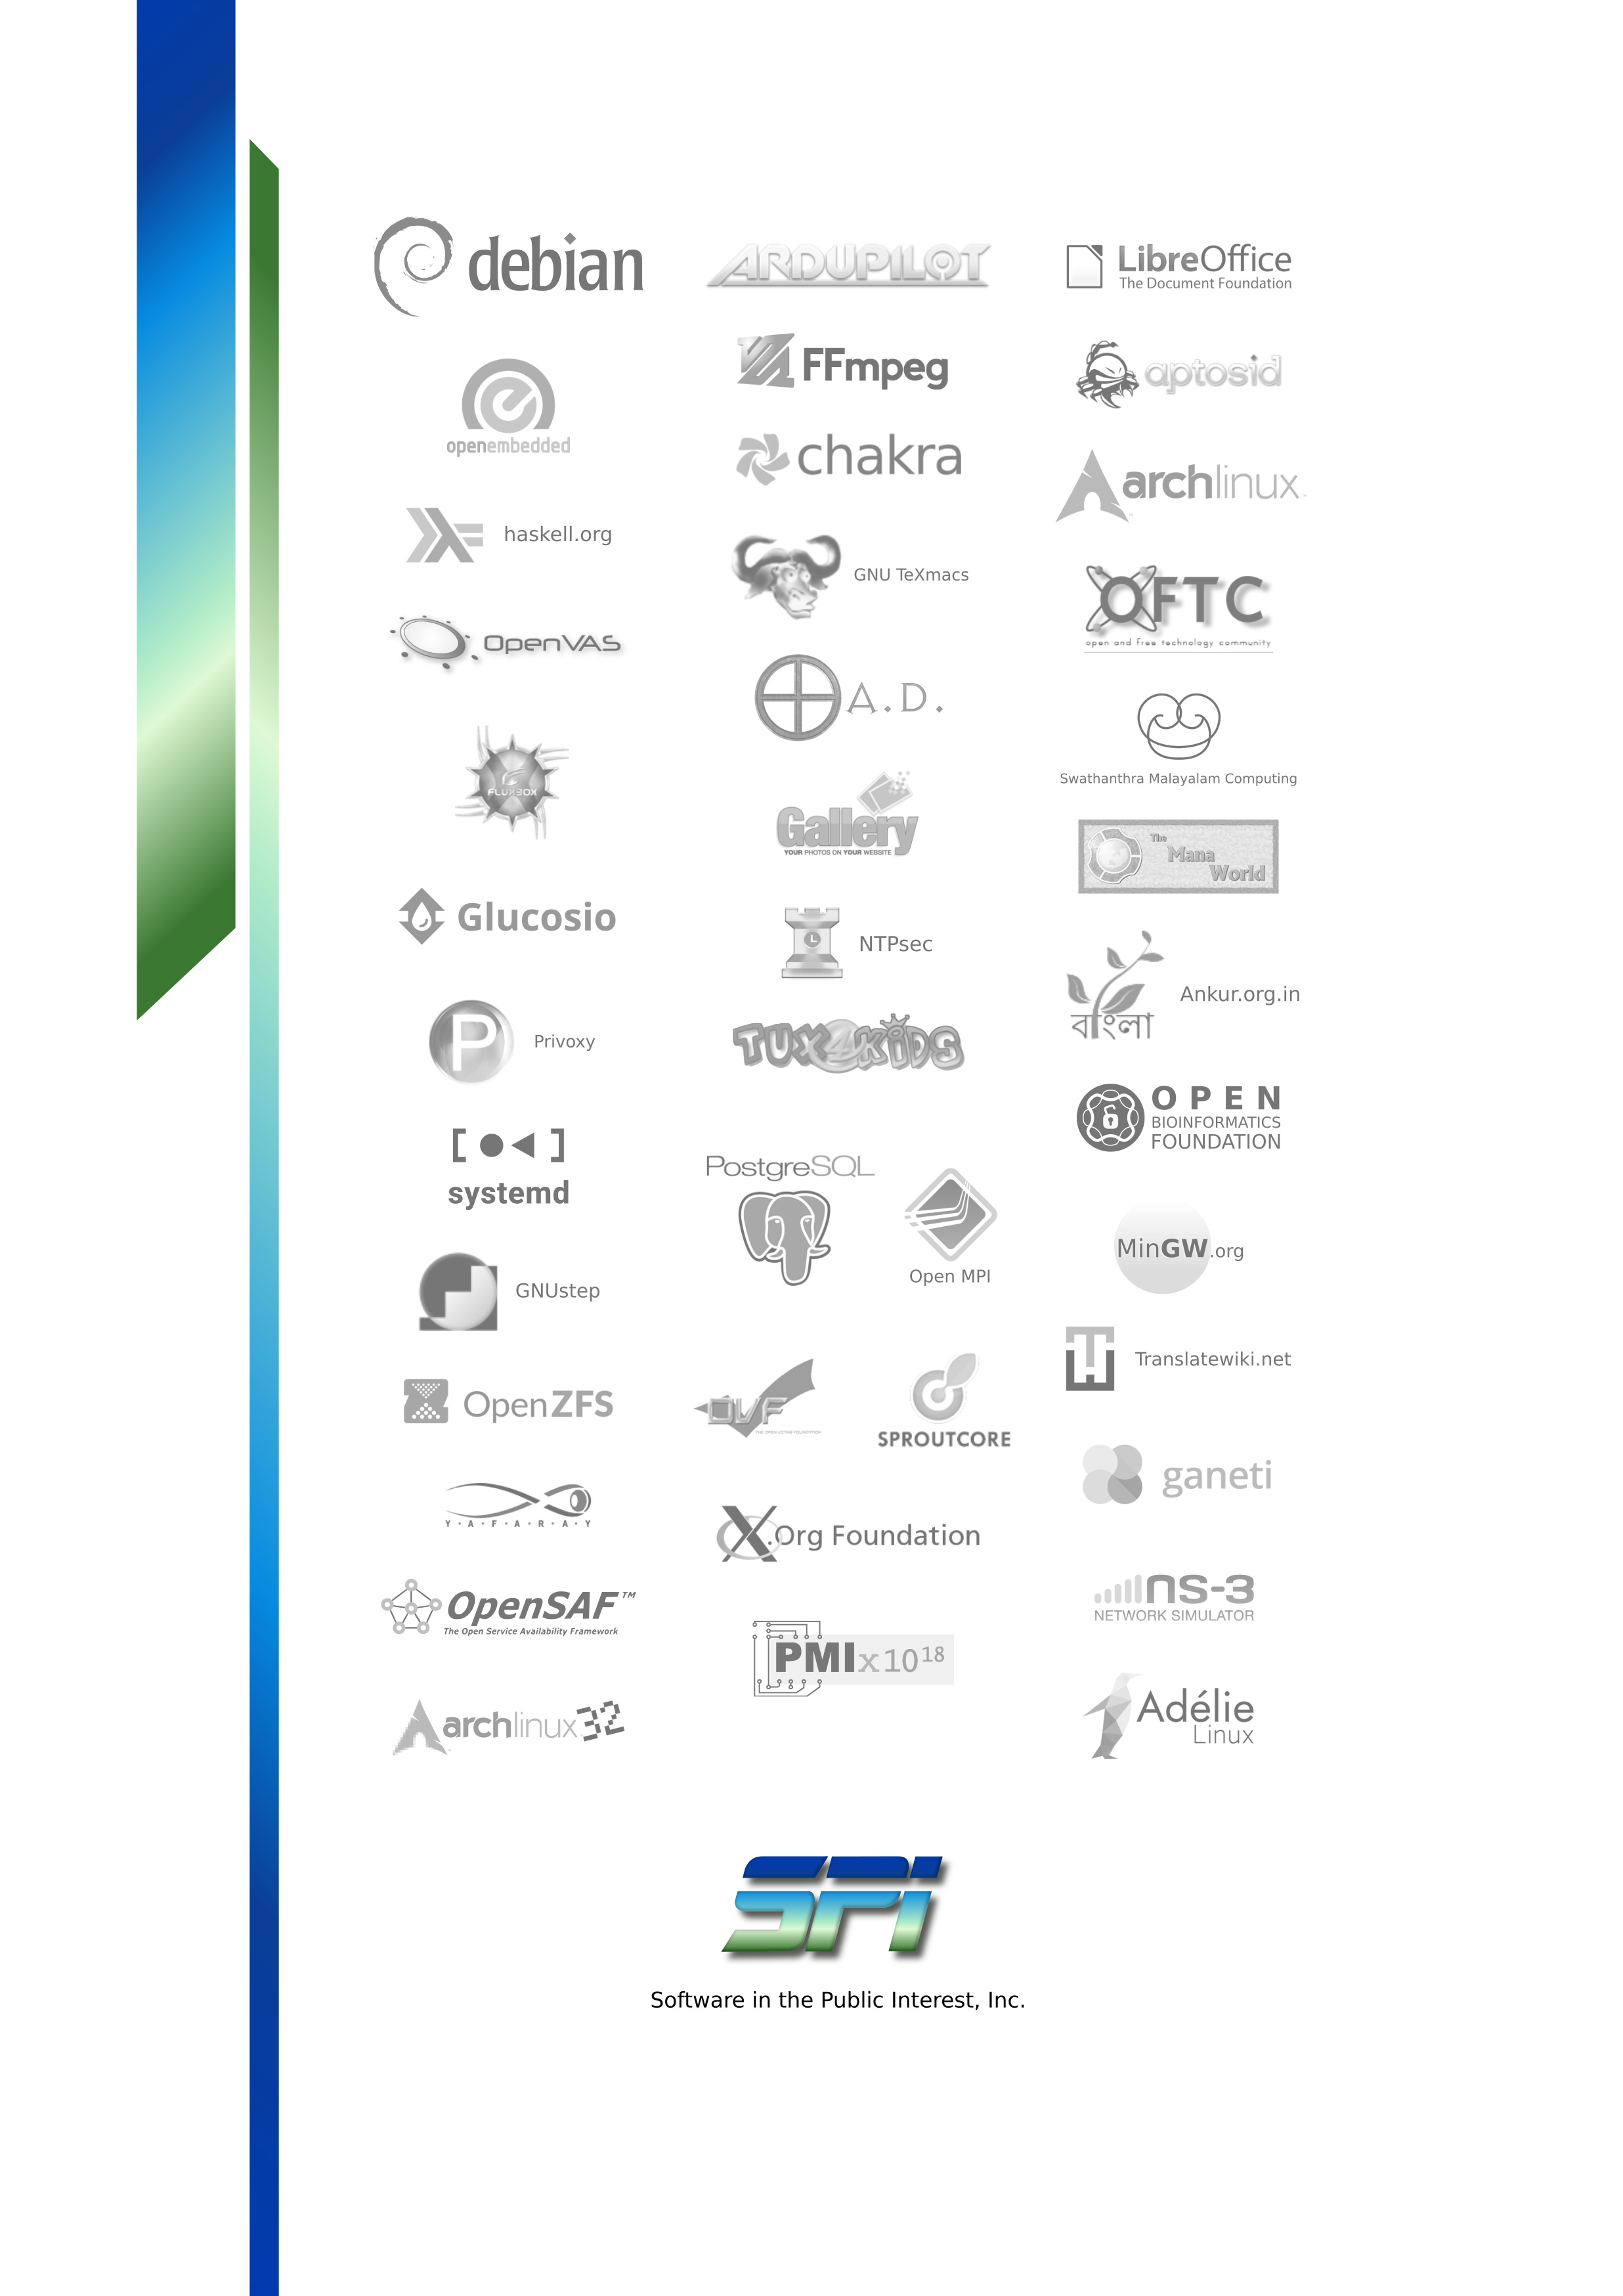
\includegraphics[width=\paperwidth,height=\paperheight]{images/spi-back-2021.jpg}}
}

\null

\end{document}
% Keep this at the bottom, thanks.
% Local Variables:
% TeX-master: "report"
% End:
